% See notation.tex for notation used throughout the paper!

%% OUTLINE (not comprehencive, notes for bits Peter & Hanbin will edit)
% Tie loose threads together of different views on relatedness,
%   in the context of the tree sequence:
%   make it precise, but easy
%   probably only biallelic markers
%   (this exists, and is about right)
% Algorithms: big-picture; details in the appendix
%   describe alg for simulating traits
%   point out matrix-vector is of a similar form
%   explain how to use matrix-vector toi efficiently do PCA

% --- INTRO TO METHODS ---------------------------------------------------

% Paragraph on The overview of methods

\subsection{ARGs and tree sequences}

% Paragraph on ARG
We first introduce our notation for ARGs, following
\citet{kelleher2016efficient, kelleher2018efficient}, and \citet{wong2023general}.
%
An ARG represents the history of a set of sampled genomes
by a collection of \emph{nodes} and \emph{edges}.
%
Each chromosome of an individual is represented by a \emph{node},
and each node has an associated \emph{time},
indicating when the individual was born.
%
In diploids, the two haploid genomes of a genotyped individual are represented
by two \emph{sample} nodes.
%
\emph{Ancestral} nodes represent genomes of non-genotyped individuals.
%
Each edge encodes the inheritance of some genome segment
by some ``child'' node from a ``parent'' node
(despite the terminology, these two may be separated by more than one generation).
%
Edges are also often referred to as \emph{branches}.
%
The \emph{span} of an edge is the length of the inherited segment of genome,
and the \emph{length} of an edge is the number of generations across which
the segment was inherited, that is, the difference between the times of parent and child nodes.
%
Genetic variation is represented in this structure
by recording where in the ARG mutations occurred.
%
For example, if we say that a mutation that produces a C nucleotide
occurs at genomic position $x$ on the edge from some parent $p$
to a child $c$, then
(1) the mutation has occurred somewhere in the chain of inheritances
by which $c$ has inherited the genetic material from $p$; and
(2) any other nodes that inherit from $c$ at position $x$ will carry a C,
unless another mutation intervenes.
%
Finally, recombination events are implicitly encoded
by edges between child and parent nodes, that is,
a child node can inherit from different nodes of different parents.
%
Inheritance relationships at each location of the genome
are described by a \emph{local tree},
and subsequent local trees are separated by the genomic locations
of recombination events.

% Paragraph on tree sequences
The \textit{succinct tree sequence}, or \textit{tree sequence} for short,
is an efficient ARG encoding \citep{kelleher2016efficient, kelleher2018efficient, wong2023general}.
%
The data structure is based on a succinct description of nodes, edges,
and mutations as described above,
and can be used to efficiently recover and process
the sequence of local trees that describe how the samples are related
on each consecutive section of the chromosome.
%
% See Figure~\ref{fig:illustration} for an illustrative diagram.

% --- TRAIT --------------------------------------------------------------

\subsection{A trait-centric notion of genetic relatedness}

% Paragraph on a trait
Consider an additive trait, that is, a trait whose value is
the sum of effects associated with each allele carried by the individual.
%
Suppose that the genotypes at each locus are from some alphabet $\mathcal{A}$,
and that at each locus $\ell$ in the genome there is an ``ancestral'' allele $a_\ell$.
%
The additive effect of allele $x$ at locus $\ell$ is $Z_{\ell,x}$,
which is relative to the ancestral allele, so that $Z_{\ell,a_\ell} = 0$.
%
More discussion of this choice can be found in Section~\ref{sec:reference_alleles} (Supplementary Material).
%
Then, an individual's genetic value is the sum of
the effects of alleles across all $n_L$ loci, % TODO: consolidate between n_{\ell} and n_L (capital for random vars)!
averaged across genome copies.
%
We will write $G_{i,\ell,g}$ for % TODO: consolidate between c and g (g is used for soo many things in genetics)!
the allele of the $g^\text{th}$ genome copy of individual $i$ at locus $\ell$,
so that a $p$-ploid individual $i$ has genetic value: % TODO: consolidate between $n_g$ and p!
%
$$
Z(i) = \frac{1}{p} \sum_{g=1}^p \sum_{\ell=1}^{n_L} Z_{\ell,G_{i,\ell,g}}.
$$
%
Finally, suppose that the effects of each non-ancestral allele $Z_{\ell,x}$
are independently drawn from a probability distribution with mean zero and variance $\sigma^2$.
%
The choice to average across genome copies (as opposed to, say, sum them)
is only consequential for situations where mixed ploidy is considered
and implies a particular model of dosage compensation or
how we summarise relatedness across genome copies.
%
Mixed ploidy arises with sex chromosomes or haplodiploids \citep{grossman1989inbreeding},
or summarizing relatedness between groups with different number of individuals \citep{cockerham1976group}.
%
Many measures of relatedness make use of this trait model (explictly or implictly),
in which case relatedness is proportional to covariance between individuals' trait values.
% proportional because we have Var(\vector{Z}) = GRM \sigma^2_z
%
We now demonstrate this equivalence.

% --- COV ----------------------------------------------------------------

For simplicity, suppose for the moment all loci are bi-allelic,
so $G_{i,\ell,g} \in \{0,1\}$, and $Z_{\ell,0} = 0$.
%
See Section~\ref{sec:multiallelic} (Supplementary Material) for a more general discussion.
%
Under this model, if we write $p(i,\ell)$ as the proportion of alleles
carried by individual $i$ at locus $\ell$ that are not ancestral
(so $p(i,\ell) = (G_{i,\ell,1} + G_{i,\ell,2})/2$ for diploids),
then the  % (usual product-moment)
covariance between the traits of individuals $i$ and $j$ is:
%
\begin{align} \label{eqn:trait_cov_non_centered}
    \Cov\left[Z(i), Z(j)\right] &= \sigma^2 \sum_{\ell=1}^{n_L} p(i,\ell) p(j,\ell) .
\end{align}
%
Note that this is the covariance of $Z(i)$ and $Z(j)$ as random variables,
averaging over random assignment of allelic effects,
but with genotypes fixed ($p(i,\ell)$ is not random).

% --- COV with invariant loci --------------------------------------------

% Paragraph on why we need to handle invariant loci differently
The above covariance expression~\eqref{eqn:trait_cov_non_centered}
depends on the choice of ancestral allele.
%
This seems undesirable for a measure of relatedness;
choosing a point farther back in time as a reference,
so that a different allele is ``ancestral'' and the derived allele is likely fixed,
should not affect relatedness within the population.
%
It does affect the relatedness calculated above because this is, implicitly,
a model of trait variation \emph{relative} to a hypothetical individual
whose genotype is composed entirely of ancestral alleles.
%
A common approach to resolve this is to \emph{center} the traits,
which takes the mean of some individuals as reference,
rather than a hypothetical ancestor.
%
When using pedigree data, these reference individuals are
founders of the pedigree \citep{wright1922coefficients},
while when using genotype data these reference individuals are
the genotyped individuals \citep{vanraden2008efficient}.

% Paragraph on centring
Suppose we have $n_I$ haploid individuals $1, \dots, n_I$
with genetic values $Z(1), \ldots, Z(n_I)$, % TODO: consolidate n_i and n_I (capital for random vars)!
and define the mean allele frequency among these individuals as
$\bar{p}(\ell) = (p(1,\ell) + \cdots + p(n_I,\ell))/{n_I}$.
%
% Again by bilinearity of covariance,
The covariance of the traits 
after centering to the sample mean is:
%
\begin{align} \label{eqn:trait_cov}
    \begin{split}
        &\Cov\left[Z(i) - \bar{Z}, Z(j) - \bar{Z}\right] \\
        &\qquad = \sigma^2 \sum_{\ell=1}^{n_L}
            \left(p(i,\ell) - \bar{p}(\ell)\right) \left(p(j,\ell) - \bar{p}(\ell)\right).
    \end{split}
\end{align}
%
If the derived allele at locus $\ell$ is fixed,
then $p(i,\ell) = \bar{p}(\ell)$ for all $i$,
and so such loci do not contribute to the covariance expression~\eqref{eqn:trait_cov}.

% Paragraph on alternative expression
It will be helpful to use another form of the mean centering
of expression~\eqref{eqn:trait_cov}.
%
If $U$ and $V$ are random, uniformly chosen individuals from the sample,
and $L$ a random, uniformly chosen locus,
then, we can rewrite $\bar Z = \E[Z(U)]$ and $\bar p(\ell) = \E[p(U,\ell)]$.
%
Consequently, the two sides of~\eqref{eqn:trait_cov}
are also equal to:
%
\begin{align} \label{eqn:trait_cov_avg}
    \begin{split}
        &\E\left[(Z(i) - Z(U))(Z(j) - Z(V)\right)] \\
        &\qquad = \sigma^2 \E\left[
            \left(p(i,L) - p(U,L)\right) \left(p(j,L) - p(V,L)\right)
        \right] ,
    \end{split}
\end{align}
%
where the expectation is averaging over choice of $U$, $V$, and $L$.
%
This rewriting in terms of an average over auxiliary random choices
can be helpful for gaining intuition or generalizing expressions.

% --- COV & GRM ----------------------------------------------------------

% Paragraph on connection between COV and GRM
The expression~\eqref{eqn:trait_cov_avg}
highlights a connection to the familiar genotype GRM.
%
Simplifying to haploids, we can treat
$\mathbf{G} \in \{0, 1\}^{n_I \times n_L}$ as the genotype matrix
for $n_I$ haploid individuals at $n_L$ loci.
%
We are interested in the covariance between individuals $i$ and $j$,
that is, between the two genomes in rows $i$ and $j$ of $\mathbf{G}$.
%
Let $\mathbf{G}^c$ be the \textit{column-centered} haplotype matrix with
entries $\mathbf{G}^c_{i,\ell} = \mathbf{G}_{i,\ell} - \mathbf{1}\bar{p}(\ell)$.
%
A common definition of covariance is:
% 
\[ \mathbf{C} = \frac{1}{n_L}\mathbf{G}^c{\mathbf{G}^c}^\intercal, \]
%
so that the covariance between individuals $i$ and $j$ based on their genotypes is:
%
\begin{align} \label{eqn:grm}
    \mathbf{C}_{i,j} = \frac{1}{n_L} \sum_{\ell=1}^{n_L} (\mathbf{G}_{i,\ell} - \bar{p}(\ell))(\mathbf{G}_{j,\ell} - \bar{p}(\ell)).
\end{align}
%
This expression~\eqref{eqn:grm} is the kernel of many variants of GRM
\citep{vanraden2008efficient, yang2010common, speed2015relatedness},
apart from difference between the haploid and diploid setting,
with the latter being an aggregate form of the former
\citep{cockerham1976group, smith1985efficient}.
%
This expression~\eqref{eqn:grm} is also equal to~\eqref{eqn:trait_cov}
divided by $n_L$, after setting $\sigma^2=1$.
%
The corresponding expression for diploids uses
in place of $\mathbf{G}$ the allelic dosage matrix
whose entries are the proportion of non-reference alleles carried by the individual.
It is more common in the literature to define the allelic dosage matrix
as the \emph{number} of non-reference alleles;
here we define it as the proportion so that it agrees with~\eqref{eqn:trait_cov};
this is necessary because 
of the convention to define $Z(i)$ as the average across the $p$ genome copies.
For diploids this results in an additional factor of four.

% --- COV 3rd time -------------------------------------------------------

% Paragraph on 3rd interpretation of COV
A third interpretation of this covariance can be derived as follows.
%
Consider two haploid individuals $i$ and $j$ and
two additional random haploid individuals $U$ and $V$ to
form the random variable $(X_i, X_j, X_U, X_V)$
that takes the value $(G_{i,\ell}, G_{j,\ell}, G_{U,\ell}, G_{V,\ell})$
with probability $\nicefrac{1}{\left({n_I}^2 n_L\right)}$
for $U, V = 1, \dots, n_I$ and $\ell = 1, \dots, n_L$.
%
In other words, we choose the individuals $U$ and $V$ uniformly at
random, with replacement, from the set of $n_I$ individuals, and
also choose a locus $\ell$ uniformly at random from the set of $n_L$ loci;
then $(X_i, X_j, X_U, X_V)$ is the alleles of those individuals at that locus.
%
In the following, we will repeatedly use the fact that
$G^2_{i,\ell} = G_{i,\ell}$ (since $G_{i,\ell} \in \{0, 1\}$).
%
Conditional on locus $\ell$, we have:
%
\begin{align*}
    \P(X_i = X_j | \ell) &= (1 - (G_{i,\ell} - G_{j,\ell})^2) \\
                         &= 1 - G_{i,\ell} - G_{j,\ell} + 2G_{i,\ell}G_{j,\ell}, \\
    %
    \P(X_i = X_U | \ell) &= \frac{1}{n_I}\sum_{u=1}^{n_I} (1 - (G_{i,\ell} - G_{u,\ell})^2) \\
                         &= \frac{1}{n_I}\sum_{u=1}^{n_I} (1 - G_{i,\ell} - G_{u,\ell} + 2G_{i,\ell}G_{u,\ell}) \\
                         &= 1 - G_{i,\ell} - p_\ell + 2G_{i,\ell}p_\ell, \\
    %
    \P(X_U = X_V | \ell) &= \frac{1}{{n_I}^2}\sum_{u=1}^{n_I}\sum_{v=1}^{n_I} (1 - (G_{u,\ell} - G_{v,\ell})^2) \\
                         &= \frac{1}{{n_I}^2}\sum_{u=1}^{n_I}\sum_{v=1}^{n_I} (1 - G_{u,\ell} - G_{v,\ell} + 2G_{u,\ell}G_{v,\ell}) \\
                         &= 1 - 2p_\ell + 2p^2_\ell.
\end{align*}
%
Combining these expressions, we have the following identity:
%
\[ 2(G_{i,\ell} - p_l)(G_{j,\ell} - p_l) = \P(X_i = X_j | \ell) -
                                           \P(X_i = X_U | \ell) -
                                           \P(X_j = X_V | \ell) +
                                           \P(X_U = X_V | \ell) .\]
% = (1 - Gi - Gj + 2GiGj) - (1 - Gi - p + 2Gip) - (1 - Gj - p + 2Gjp) + (1 - 2p + 2p^2)
% = 1 - Gi - Gj + 2GiGj - 1 + Gi + p - 2Gip - 1 + Gj + p - 2Gjp + 1 - 2p + 2p^2
% = (1 - 1 - 1 + 1) --> 0
%   (-Gi + Gi) --> 0
%   (-Gj + Gj) --> 0
%   (p + p - 2p) --> 0
%   (2GiGj - 2Gip - 2Gjp + 2p^2)
% = 2(GiGj - Gip - Gjp + p^2)
% = 2(Gi - p)(Gj - p)
%
Note the similarity to expression~\eqref{eqn:trait_cov_avg}.
Since $\ell$ is chosen uniformly at random, it follows that:
%
\small{
\begin{align} \label{eqn:cov_prob}
    \mathbf{C}_{i,j} = \frac{1}{2}\left(\P(X_i = X_j) - \P(X_i = X_U) - \P(X_j = X_V) + \P(X_U = X_V) \right).
\end{align}
}
This expression is more readily extendable to multi-allelic data.

% Paragraph on three expressions
We therefore have the following three equivalences
(\ref{eqn:trait_cov}, \ref{eqn:grm}, and \ref{eqn:cov_prob}):
%
\begin{align} \label{eqn:equivalence}
    \mathbf{C}_{i,j} &= \frac{1}{n_L \sigma^2}\Cov\left[Z(i) - \bar{Z}, Z(j) - \bar{Z}\right] \tag{\ref{eqn:trait_cov}} \\
                     &= \frac{1}{n_L}\sum_{\ell=1}^{n_L} (G_{i,\ell} - p_\ell)(G_{j,\ell} - p_\ell) \tag{\ref{eqn:grm}} \\
                     &= \frac{1}{2}\left(\P(X_i = X_j) - \P(X_i = X_U) - \P(X_j = X_V) + \P(X_U = X_V) \right) \tag{\ref{eqn:cov_prob}}.
\end{align}
%
From the third equivalence~\eqref{eqn:cov_prob},
the quantity $n_L\mathbf{C}_{i,j}$ has the following interpretation.
%
Let $m(i,j)$ denote the number of pairwise allele matches between
the individual $i$ and $j$,
and let $U$ and $V$ be independently chosen individuals from the set of individuals.
%
Then the quantity $n_L\mathbf{C}_{i,j}$
is the expected number of pairwise allele matches between $i$ and $j$
relative to the rest of individuals:
%
\begin{align} \label{eqn:relative_allele_matches}
    n_L \mathbf{C}_{ij} = \E[m(i,j) - m(i,U) - m(j,V) + m(U,V)],
\end{align}
%
where the expectation is over the choice of U and V.
%
This interpretation is closely related to the definition of kinship
between individuals $i$ and $j$ as the
``the probability of a match between alleles drawn at random from each of them'',
averaged over loci, and with the alleles drawn with replacement if $i=j$
\citep{malecot1969mathemathics, speed2015relatedness}.
%
See also \citet{weir2017unified, weir2018how} and \citet{ochoa2021estimating} on
other ``relative'' kinship estimators.

% --- Branch relatedness ----------------------------------------------

\subsection{A trait-centric perspective on the branch relatedness} \label{sec:trait-centric}

% Paragraph on branch relatedness
We now describe a closely related notion of branch relatedness.
%
Suppose that we only observe the relationships in the ARG,
not the mutations that appear in it.
%
This is similar to the starting point of pedigree relatedness,
but we assume we also know full ancestry of each genome all the way to the roots
of each local tree (the MRCAs) and
which portions of the genomes were inherited in each relationship.
%
The expected number of mutations that appear on a segment of genome of $s$ base pairs
inherited across $b$ generations is proportional to $b \times s$.
%
In other words, the expected number of mutations on an edge of length $b$ and span $s$
is proportional to its area, $A = b \times s$.
%
If the effect of each mutation has variance $\sigma^2$,
then the variance of the edge effect is $A \sigma^2$.
%
(This is because the variance of the sum of a random number $N$ of
independent and identically distributed mean-zero terms is
the mean of $N$ multiplied by the variance of the terms.)
% Note: this is, counter-intuitively, quite general, because
% $\var[\sum^N X_i] = \E[\var[\sum^N X_i|N]] + \var[\E[\sum^N X_i|N]] = \E[N]\var[X] + \var[N]\E[X]$ .
%
Let $A(i,j)$ be the total area of branches ancestral to individuals $i$ and $j$.
%
Then, just as above, with randomly chosen individuals $U$ and $V$:
%
\begin{align} \label{eqn:branch_cov}
    \mathbf{B}_{i,j}
         &=\Cov\left[Z(i) - \bar{Z}, Z(j) - \bar{Z}\right] \notag \\
         &= \E[A(i,j) - A(i,U) - A(j,V) + A(U,V)] , 
         % &= \frac{1}{n_I^2} \sum_{k=1}^{n_I} \sum_{\ell=1}^{n_I} \left(A(i,j) - A(i,k) - A(i,\ell) + A(k,\ell)\right)
\end{align}
%
where the expectation in the second line is over the choice of $U$ and $V$,
while $Z(i)$ and $\bar{Z}$ are defined as before.
%
Note that the random variables $Z(i)$ are the same as before,
but this expression differs from~\eqref{eqn:trait_cov} in that
here the covariance averages not only over allelic effects,
but also over location of the mutations.
%
This is an example of a general relationship described in \citet{ralph2020efficiently}.

% Paragraph on branch GRM and coalescence times
The branch relatedness can also be rewritten as a weighted average of coalescence times,
as noted by \citet{mcvean2009genealogical, fan2022genealogical}, and \citet{zhang2023biobank}.
%
Let $s_k$ be the genome sequence length corresponding to the $k^\text{th}$ local tree,
and within this tree define
$b(i,j,k)$ be the total length of branches ancestral to both haploid individuals $i$ and $j$, $t(i,j,k)$
be the TMRCA of $i$ and $j$, and $\hat{t}(k)$ the time of the root.
%
Supposing that $i$ and $j$ are both at time 0,
then the time of the root is equal to the TMRCA plus any additional, shared, branch lengths:
%
\begin{align} \label{eqn:branch_relations}
    \hat{t}(k) = b(i,j,k) + t(i,j,k) .
\end{align}
%
We can use this relationship to split~\eqref{eqn:branch_cov} by local tree as follows:
%
\begin{align}
    \mathbf{B}_{i,j}
        % &\qquad = \sum_{k = 1}^{n_T}        \E[A(i,j,k) - A(i,U,k) - A(j,V,k) + A(U,V,k)] a\
        & = \sum_{k = 1}^{n_T} s_k \E[b(i,j,k) - b(i,U,k) - b(j,V,k) + b(U,V,k)] \\
        & = \sum_{k = 1}^{n_T} s_k \E[t(i,U,k) + t(j,V,k) - t(i,j,k) - t(U,V,k)],
\end{align}
%
where $n_T$ is the number of local trees in the ARG, % TODO: change $n_T$ to $n_k$ since t is time?
and the expectation averages over $U$ and $V$.

% Paragraph on eGRM and branch GRM
Our definition differs slightly from the eGRM by \citet{fan2022genealogical}
%
Let $S_{i,e,k} = 1$ if sample $i$ is a descendant of branch $e$
in the $k^\text{th}$ tree and $S_{i,e,k} = 0$ otherwise,
and $\bar{S}_{e,k} = \sum_{i=1}^{n_I} S_{i,e,k} / n_I$
for the proportion of samples inheriting from $e$.
Also, write $b_e$ for the length of $e$.
%
Then~\eqref{eqn:branch_cov} can be rewritten as:
\begin{align*}
    \mathbf{B}_{i,j}
    = \sum_{k=1}^{n_T} s_k \sum_{e \in T_k} b_e (S_{i,e,k} - \bar{S}(e,k))(S_{j,e,k} - \bar{S}(e,k)) ,
\end{align*}
where the second sum is over edges $e$ in the $k^\text{th}$ tree.
%
On the other hand, \citet{fan2022genealogical} define the eGRM as:
%
\begin{equation}
    eGRM_{i,j}
    = \frac{1}{A_T} \sum_{k=1}^{n_T} s_k \sum_{e \in T_k} b_e \frac{
        (S_{i,e,k} - \bar{S}(e,k))(S_{j,e,k} - \bar{S}(e,k)) 
        }{
        \bar{S}(e,k) (1 - \bar{S}(e,k))
        } ,
\end{equation}
where $A_T = \sum_k \sum_{e \in T_k} s_k b_e$ is the total area of the ARG.
%
The different denominator normalises the contribution of each edge according to its standard deviation in the population,
and is equivalent to the $\sqrt{2p(1-p)}$ standardization often used in the genotype GRM.

% Paragraph on relatedness and divergence
Relatedness and divergence are closely related,
as demonstrated by the relationship~\eqref{eqn:branch_relations}.
%
Let $d(i,j,k)$ be the distance in the $k^\text{th}$ tree between $i$ and $j$,
and $r_k$ the root of the $k^\text{th}$ tree.
%
A more general relationship that does not assume $i$ and $j$ are both at time zero is
\citep{semple2003phylogenetics}:
%
\begin{align}
    d(i,r_k,k) + d(j,r_k,k) = 2 b(i,j,k) + d(i,j,k) .
\end{align}
%
That is, the sum of the distances from each to the root is
equal to the distance between them plus twice the distance from their MRCA to the root.
%
Let $R(i)$ denote the sum along the genome of the distances from $i$ to the root and
$D(i,j)$ the sum along the genome of the distances between $i$ and $j$ in the local trees.
%
Then $D(i,j)$ is the branch genetic divergence between $i$ and $j$ \citep{ralph2020efficiently},
and summing the previous relation across the genome, we get:
%
\begin{align} \label{eqn:divergence_relatedness}
    R(i) + R(j) = 2 A(i,j) + D(i,j) .
\end{align}
%
Rearranging and substituting into the expression for branch relatedness~\eqref{eqn:branch_cov},
centering cancels the terms with $R$, giving:
%
\begin{align}\label{eqn:divergence_relatedness_branch}
    \mathbf{B}_{i,j} = - \frac{1}{2} \E[D(i,j) - D(i,U) - D(j,V) + D(U,V)] .
\end{align}
%
Thought of as matrices, if $\mathbf{P}=\mathbf{I} - \mathbf{1}\mathbf{1}^\intercal / n_I$ is the $n_I \times n_I$
centering matrix, the above equation says that $\mathbf{B} = - \mathbf{P} \mathbf{D} \mathbf{P} / 2$.
% A more usual way to write this would be
% \begin{align*}
%     \mathbf{B}_{i,j} = - \frac{1}{2} \left(
%         D(i,j)
%         - \frac{1}{n_I} \sum_{k=1}^{n_I} (D(i,k) + D(j,k))
%         + \frac{1}{n_I^2} \sum_{k=1}^{n_I} \sum_{\ell=1}^{n_I} D(k,\ell)
%     \right) .
% \end{align*}

\subsection{Branch PCA}

Principal component analysis (PCA) is a commonly used technique to quantify and visualise population structure from genotype data. Mathematically, PCA operates by projecting samples onto a set of orthogonal axes, each defined as a linear combination of genotype values across SNPs or other genetic variants. An iterative characterization of PCA is as follows: choose the first principal component to be the axis that captures the maximum possible variance in the data, then choose the second principal component that maximizes variance whilst being orthogonal to the first, and so on. The first three or four principal components are often presented as a low-dimensional summary of population structure.

Equivalent ways to undertake PCA is
to compute the eigenvectors of the (centered) genotype GRM or
to compute singular value decomposition (SVD) of underlying (centered) genotype matrix.
Both use powerful linear algebra techniques that focus on computing a subset of the principal components.
These decomposition can be efficiently approximated with randomized algorithms that can operate on
dense matrices or on implicitly defined matrix-vector products \citep{halko2011findingstructure}.
\citet{mcvean2009genealogical} gave a genealogical interpretation of PCA, while
\citet{fan2022genealogical} showed that branch PCA can better capture recent population structure than genotype PCA,
even when based on the same genotype information.
These developments indicate an alternative approach to characterizing population structure,
either through dense branch GRM or implicitly defined branch GRM-vector product.
In sub-section~\ref{subsec:matvec} we describe an efficient algorithm for
such a product that bypasses the construction of branch GRM
and operates directly on tree sequence encoding of an ARG.
However, we first connect and demonstrate pedigree and branch relatedness.

\subsection{Connection between pedigree and branch relatedness}

The pedigree relatedness of two individuals in a given pedigree is
the probability that they both inherit from the same ancestral genomes within the pedigree,
that is, that they are IBD within the pedigree \citep{malecot1969mathemathics}.
%
While pedigree and branch relatedness seem similar,
they in fact differ in what they measure.
%
Using IBD to define an ARG-based notion of relatedness would lead to an ``IBD GRM''
as defined by~\citet{tsambos2022efficient}.
%
While the IBD relatedness measures the
probability of identity with reference to a particular time (or set of ancestors) in the past,
branch relatedness measures shared edge area.
%
This difference in units is confusing given the correspondence between
the expressions~\eqref{eqn:cov_prob} and~\eqref{eqn:branch_cov}.
%
Because branch relatedness $\mathbf{C}_{i,j}$ can be written using probabilities of identity,
it seems analogous to IBD relatedness within a pedigree or an ARG,
but the close theoretical relationship to $\mathbf{B}_{i,j}$
tells us that it is better to think about branch relatedness as having units of ``shared time''.

% --- FRENCH-CANADIANS --------------------------------------------------------

\subsection{Demonstration with the French-Canadian pedigree}

To empirically illustrate the connection between pedigree and branch GRM,
we analysed the pedigree of a subset of 2,321 probands from the BALSAC dataset,
drawn from five different regions in Quebec (Figure~\ref{fig:PCA_map}G).
%
For this subset, we computed pedigree and branch GRM.
%
For the latter, we obtained an ARG from pedigree- and ancestry-informed simulation
and computed branch GRM from the ARG.
%
We simulated 100 such ARGs to evaluate the variance in branch GRM within a fixed pedigree.
See Methods for more details on the dataset and simulations performed.

%\subsubsection{Principal components analyses}

\begin{figure}
    \centering
    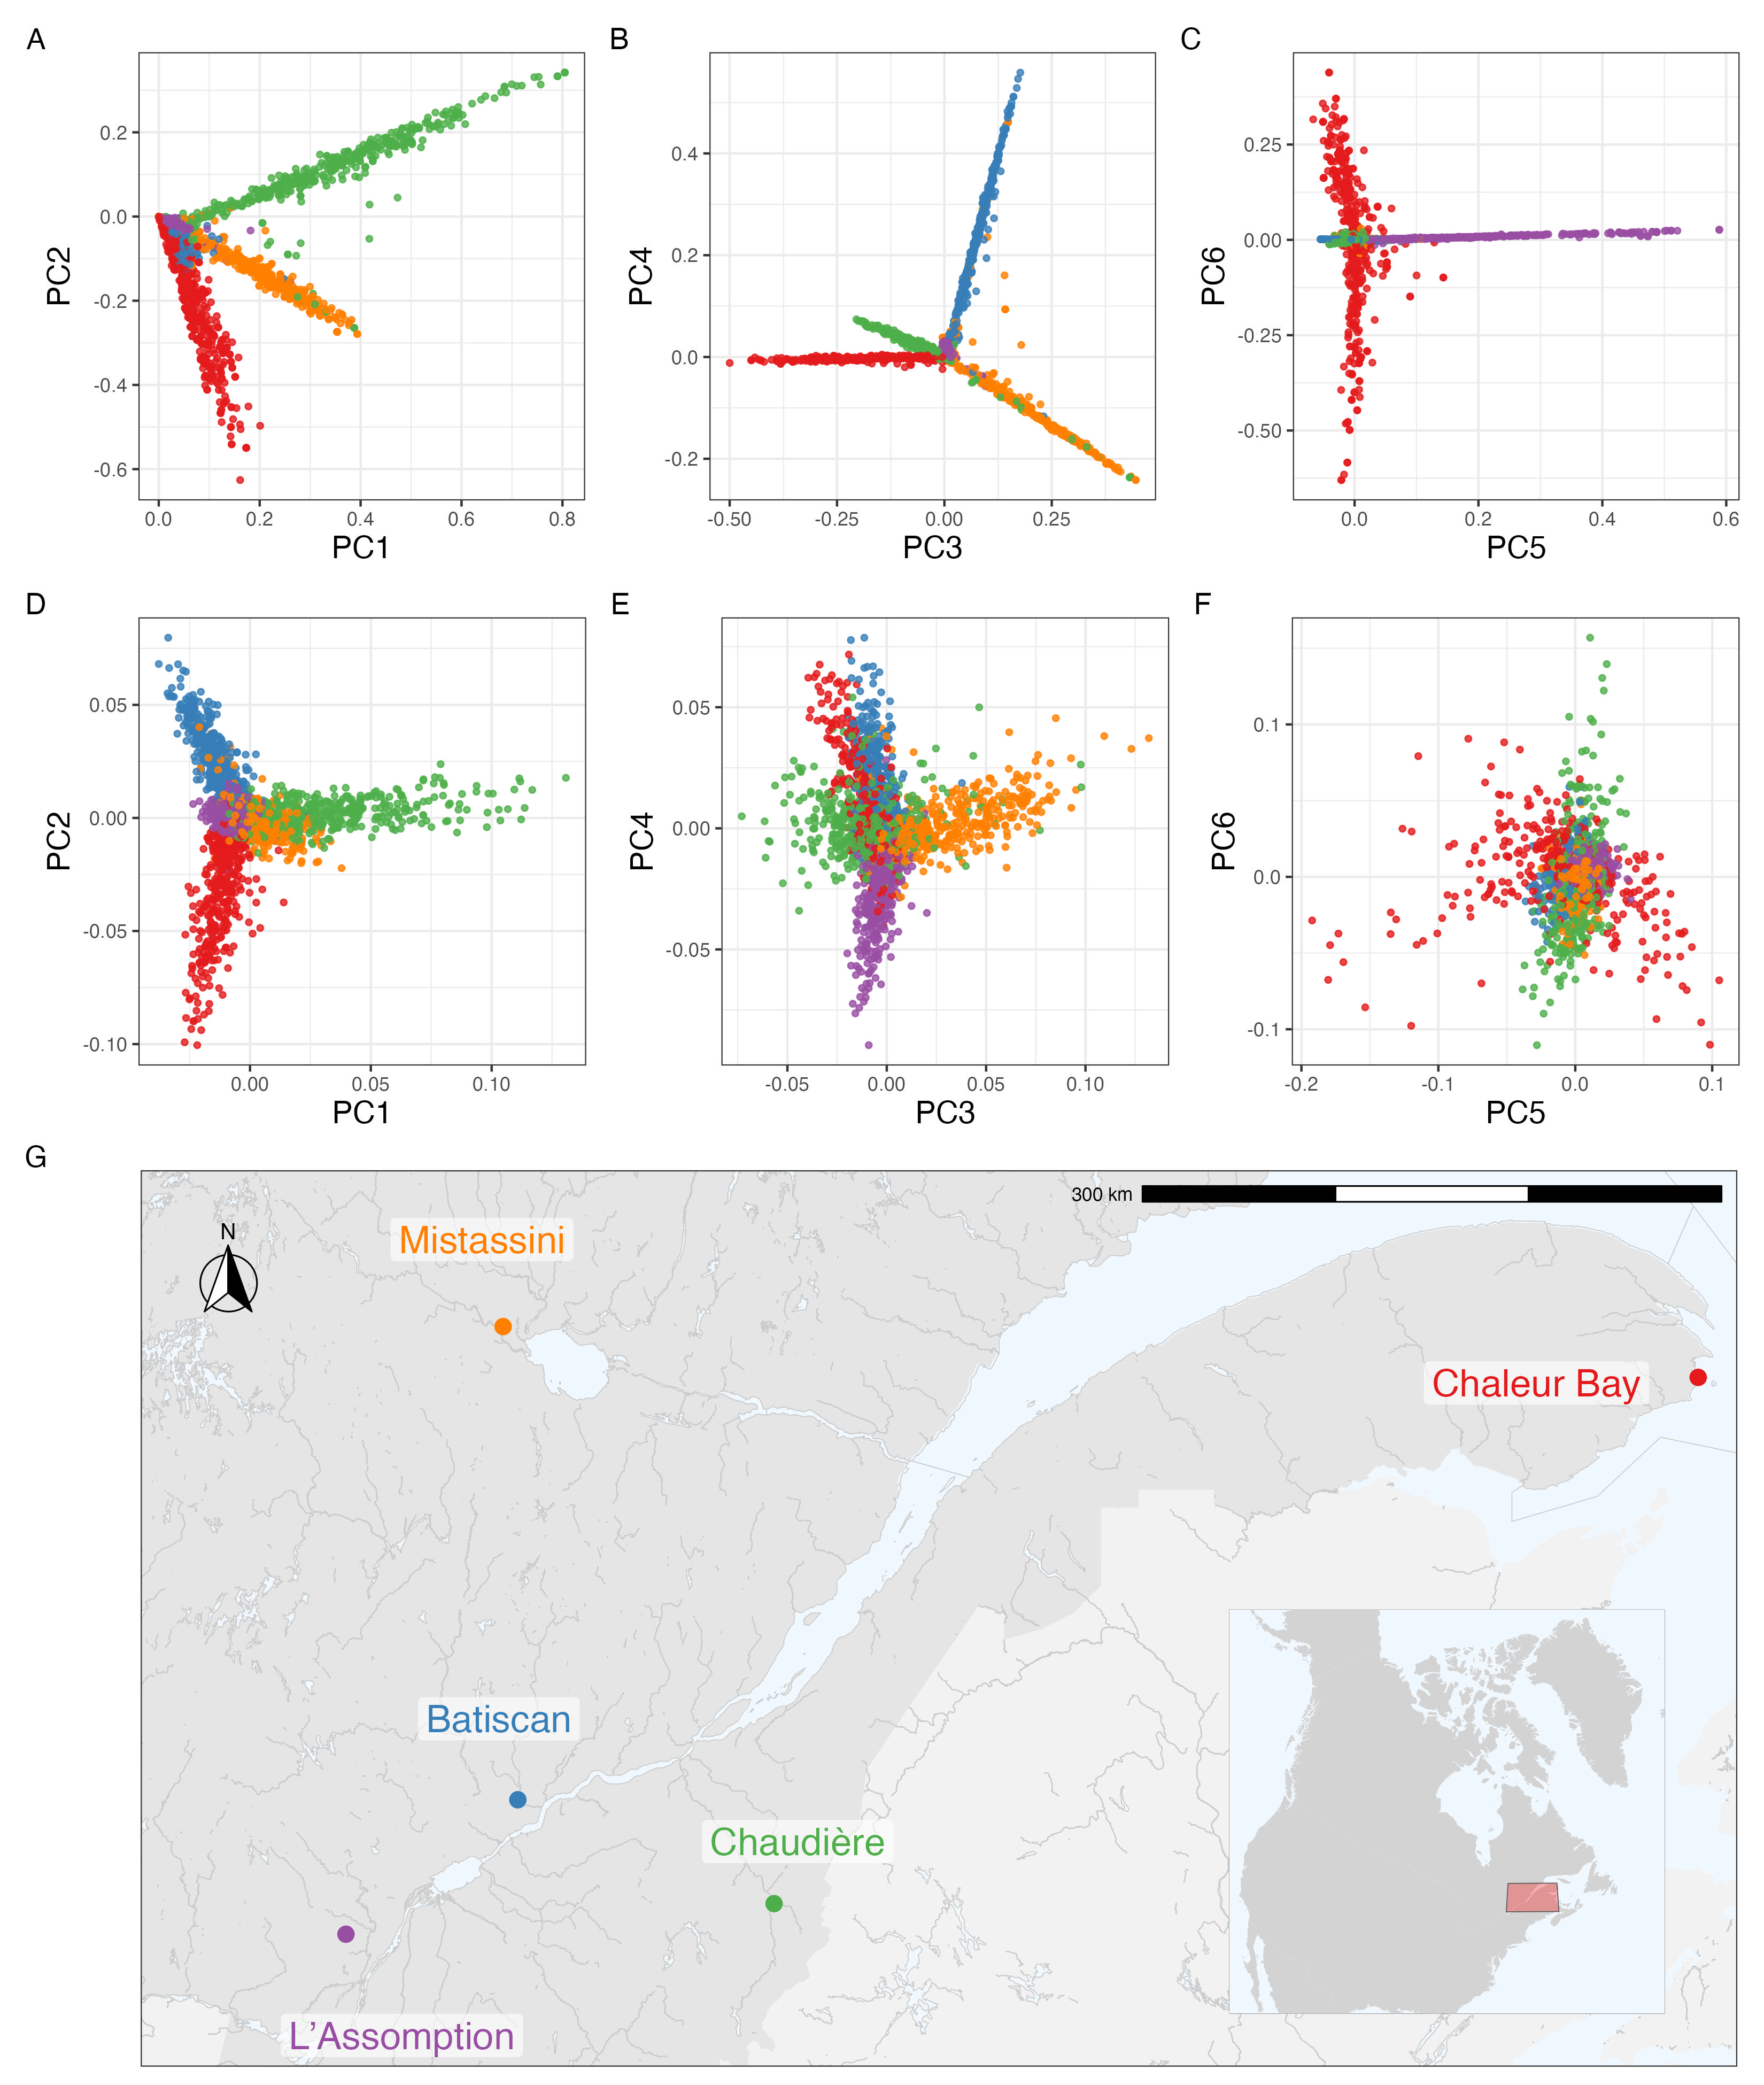
\includegraphics[width = \textwidth]{Figures/map_and_pca_grid4.jpg}
    \caption{Principal components analysis of pedigree and branch GRM of French-Canadian individuals.
    (A-C) The first six principal components of pedigree GRM.
    (D-F) The first six principal components of branch GRM.
    (G) A partial map of Quebec with approximate locations of sampled individuals. \label{fig:PCA_map}}
\end{figure}

% Paragraph on pedigree PCs
The overall population structure according to pedigree and branch PCA
of the 2,321 probands is shown in Figure~\ref{fig:PCA_map}
with noticeable clustering by the five regions.
%
The pedigree PCs show sharp distinctions between individuals from different regions
(Figure~\ref{fig:PCA_map}A-C).
%
Although individuals from each of the regions share a common bottleneck,
over the last four centuries,
each of the regions have drifted in their own unique way
leading to each region pulling a distinct principal component.
%
PCs 1 and 2 show a clear structure between individuals from Chaudière, Chaleur Bay, and Mistassini.
%
PCs 3 and 4 distinguish between individuals of each of the five regions except L'Assomption.
%
PCs 5 and 6 illustrate a clear distinction between L'Assomption and Chaleur Bay.
%
Only a few individuals deviated from the clusters.

% Paragraph on branch PCs
The branch PCs also show the population structure (Figure~\ref{fig:PCA_map}D-F),
but there are at least two notable differences compared to pedigree PCs.
%
First, some regions clustered differently with branch PCs than with pedigree PCs.
%
This difference could be because branch PCs are based on the ARG,
which captures deeper ancestry than the pedigree,
however due to the shared bottleneck and pedigree missingness
further research is needed to study the source of these differences.
%
Second, branch PCs show more variation than pedigree PCs.
%
%This higher variation is partly because we have used one simulated ARG (for one chromosome) for the branch GRM, leading to a high variance in branch PCs, but again also because of deeper ancestry encoded in the ARG, which pedigree does not capture.
This higher variation is due to the randomness of genetic inheritance within a single chromosome, which is not reflected in the pedigree \citep{weir2006genetic, hill2011variation, thompson2013identity, garciacortes2013variance}.
%
This variability is also evidenced when comparing relatedness between a subset of 250 individuals: a clearer structure emerges with pedigree GRM than with branch GRM (Figure~\ref{fig:grm_heatmap}).
% 
%\todo[inline]{Brieuc: Confim/check/rewrite this sentence (on the one ARG used for branch GRM}
%
% When we have computed branch GRM across 23 simulated ARGs (for 23 chromosomes) within the fixed pedigree,
% the variance in corresponding branch PCs decreased (Figure~\ref{fig:PCA_map}G-I / \ref{fig:PCA_map23}).
%
%\subsubsection{Comparing pedigree and branch GRM}
%Comparison of relatedness between 250 French-Canadian i
%The difference between the two GRMs is stark due to the randomness of genetic inheritance for a single chromosome, which is not captured by pedigree.
%
% When branch GRM is computed across 23 simulated ARGs (for 23 chromosomes) within the fixed pedigree,
% the similarity between the pedigree and branch GRMs increased (Figure~\ref{fig:grm_heatmap23}).
%
Notably, when individuals have a shallow pedigree
(for example, one sampled individual from Chaleur Bay),
their corresponding pedigree GRM rows and columns have low pedigree relatedness,
while this is not the case with branch relatedness.

\begin{figure}
    \centering
    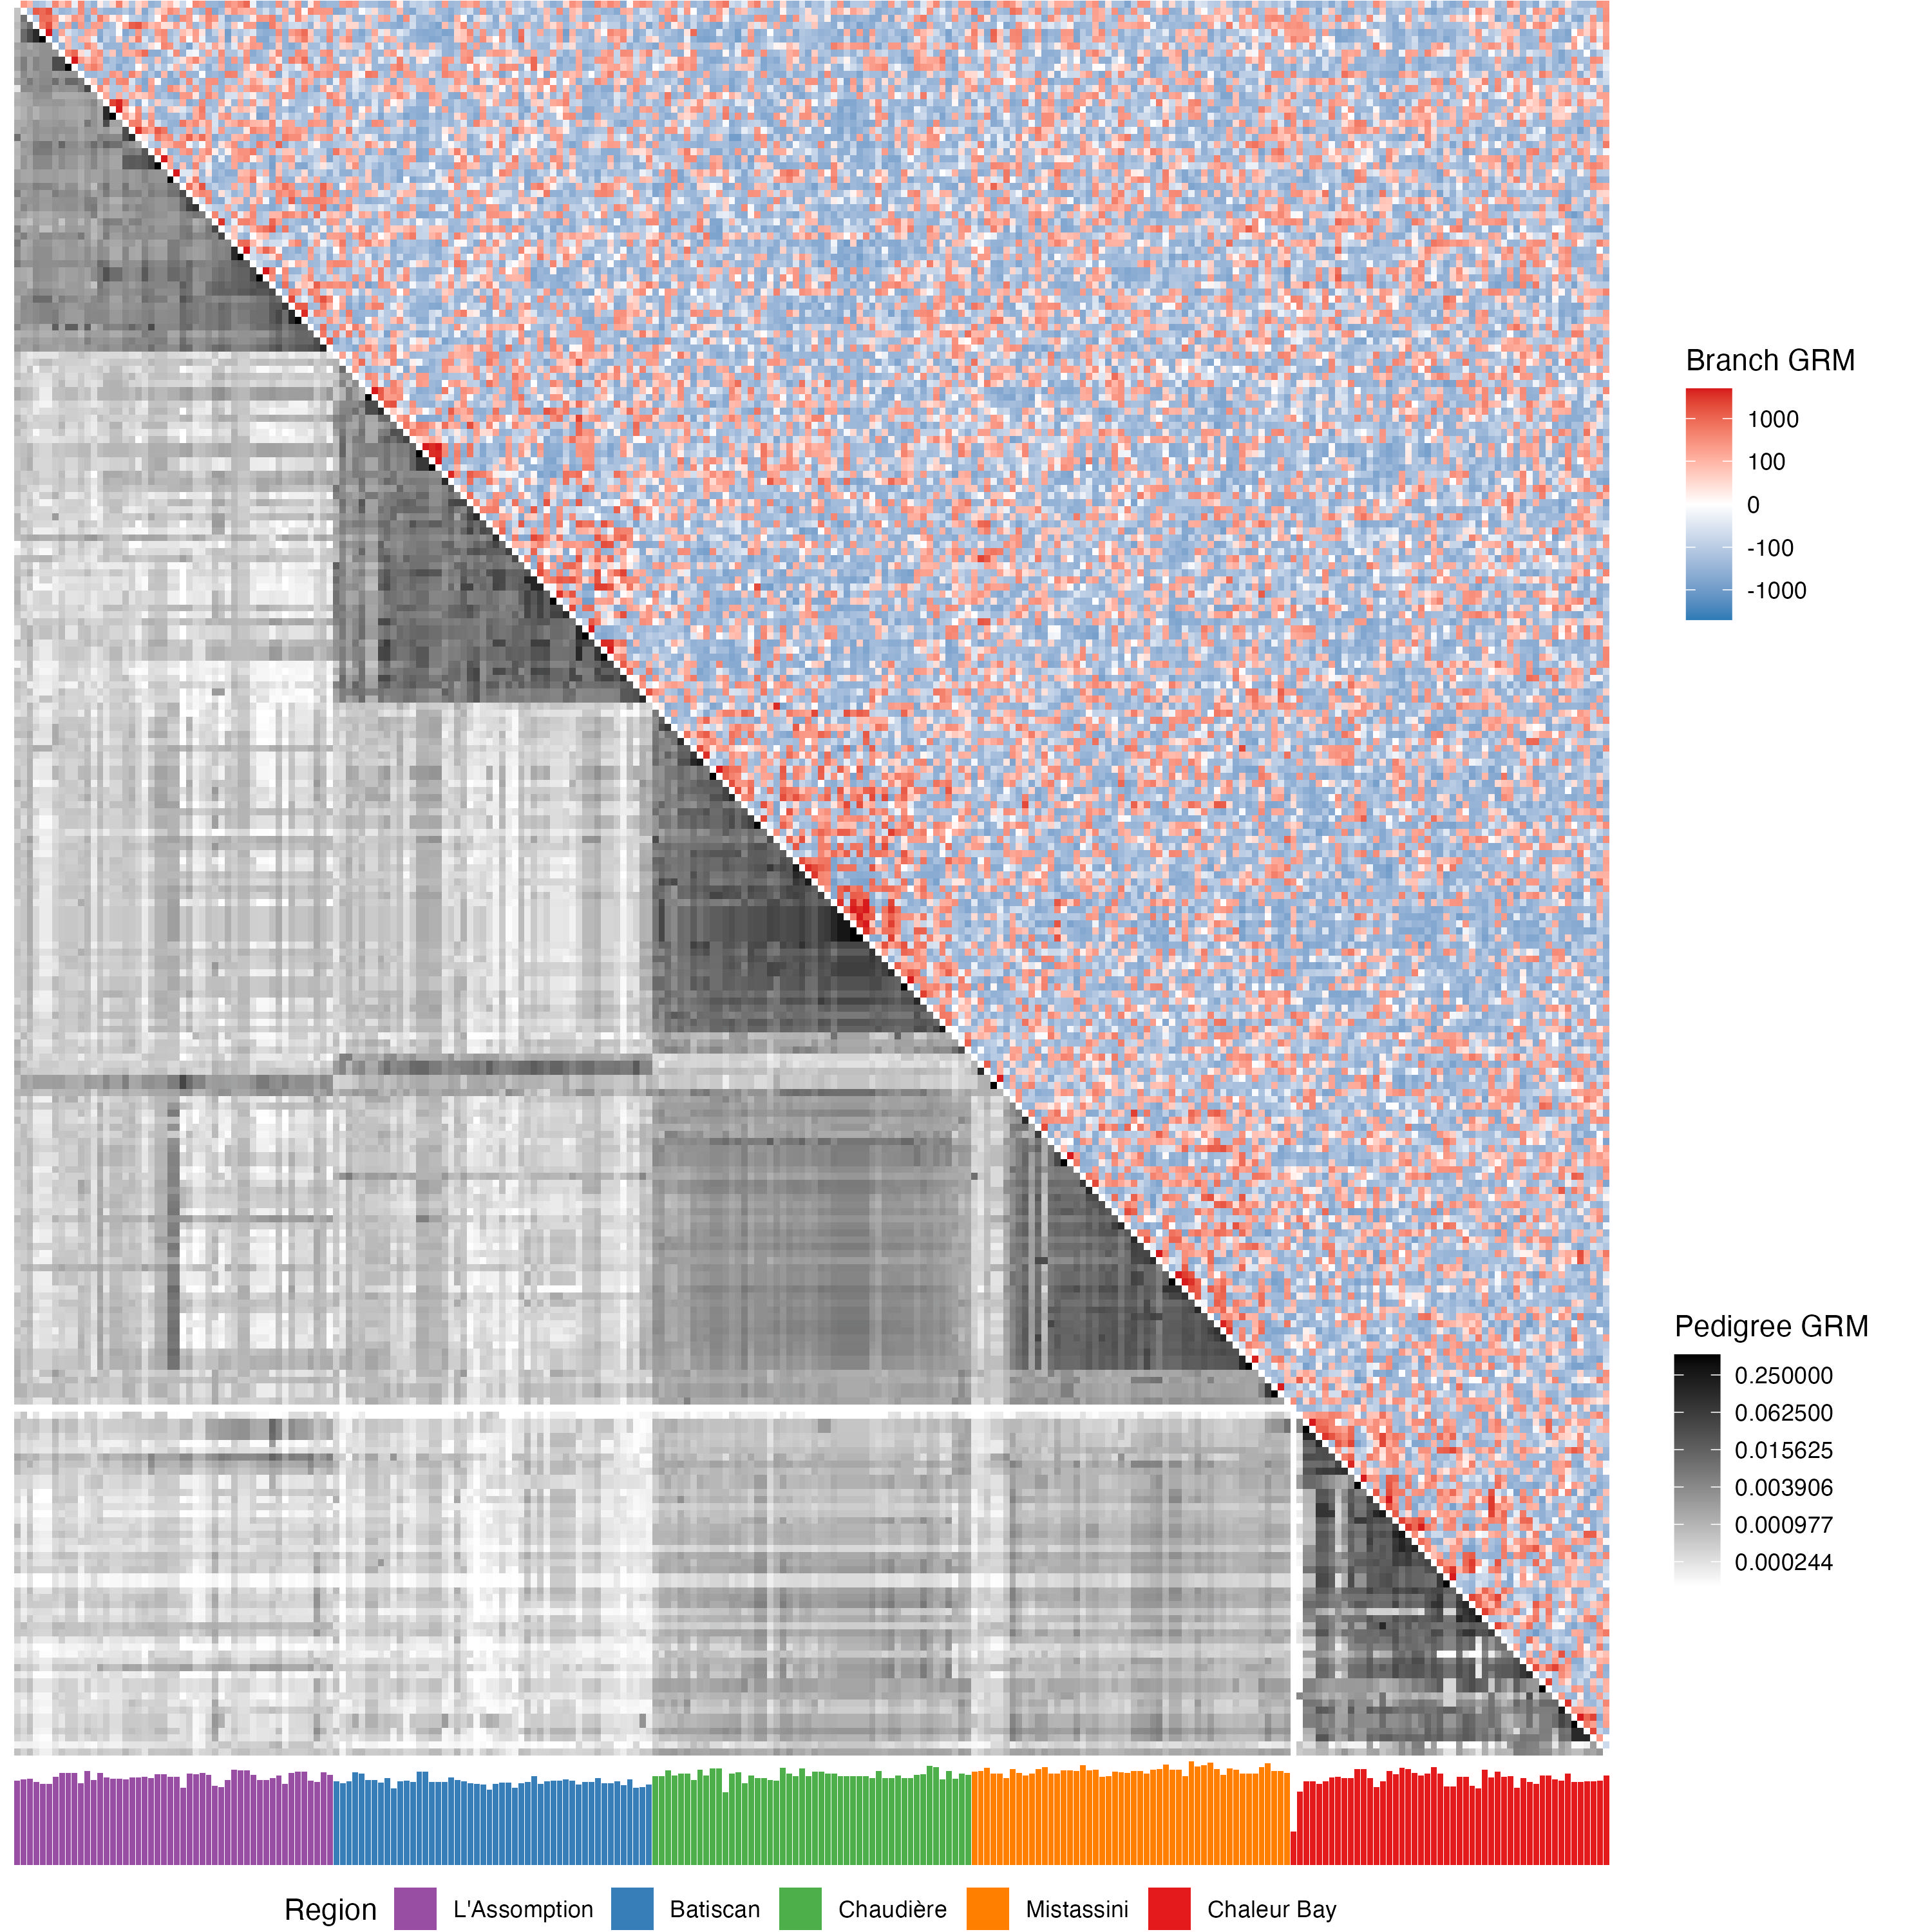
\includegraphics[width=\textwidth]{Figures/Fig4_grm_prm_heatmaps4.jpg}
    \caption{Relatedness between 250 French-Canadian individuals from 5 regions in Quebec.
      Upper-triangle: Heatmap of the branch GRM computed from one ARG (one chromosome).
      Lower-triangle: Heatmap of the pedigree GRM. 
      Bottom: Barplot of the average founder depth in the pedigree for each individual.
      The ordering of individuals is based on region and within region hierarchically on pedigree GRM.
      Because of the log scaling in the heatmap of branch GRM, we used an epsilon of 1e-4 to avoid issues with values close to zero.
    }
    \label{fig:grm_heatmap}
\end{figure}

%\subsubsection{Variability in branch GRM within a fixed pedigree}

% Paragraph on main relationship between branch and pedigree relatedness
Next, we explored the variability in branch relatedness across the 100 simulated ARGs
(Figure~\ref{fig:boxplots}).
%
As expected, the branch relatedness increases with pedigree relatedness.
%
Since pedigrees are often shorter than the mean TMRCA,
and so the contribution of branch lengths within the pedigree is small,
a simple approximation of the relationship between the two
can be derived as follows.
%
First, since pedigree relatedness $r_{i,j}$ between a pair of individuals
is the expected proportion of the genome on which the two inherit from
a common ancestral genome within the pedigree,
we expect branch relatedness $C_{i,j}$ to be $r_{i,j} C_0 + (1 - r_{i,j}) C_*$,
where $C_0$ is the average branch relatedness of a genome to itself in pedigree founders,
and $C_*$ is the average branch relatedness of two distinct genomes from the pedigree founders.
%
Since this relatedness is \emph{centered}, we can (very roughly) take
$C_* \approx 0$ and $C_0 \approx A(U,U) - A(U,V)$ (with $U$ and $V$ random individuals).
%
In other words, the average centered branch relatedness
of a typical genome to itself is the total area of edges back to the roots,
minus shared edges between two typical (but different) genomes.
%
Using the relationship~\eqref{eqn:divergence_relatedness},
this is $C_0 \approx D(U,V)/2$.
%
Hence, we expect $\mathbf{B}_{i,j} \approx r_{i,j} T$
where $T$ is the mean TMRCA for two random samples from the population
(computable as one half of branch genetic divergence in \tskit{}).
%
This is shown with a line in Figure~\ref{fig:boxplots},
with $T$ computed from the demographic model used for recapitation of the pedigree.

% Paragraph on variance in branch relatedness compared to pedigree relatedness
However, there is a degree of variability in branch relatedness
between different pairs of individuals with similar pedigree relatedness.
%
While branch relatedness broadly tracks the expected relatedness outlined above,
it varies around this value across the range of pedigree relatedness.
%
Moreover, there is substantial variability in branch relatedness across one chromosome
for a pair of individuals.
%
This variability is highest for sibling pairs and decreases with pedigree relatedness.
%
We expect the absolute variability to decrease when considering
branch relatedness across the whole genome.

\begin{figure}
    \centering
    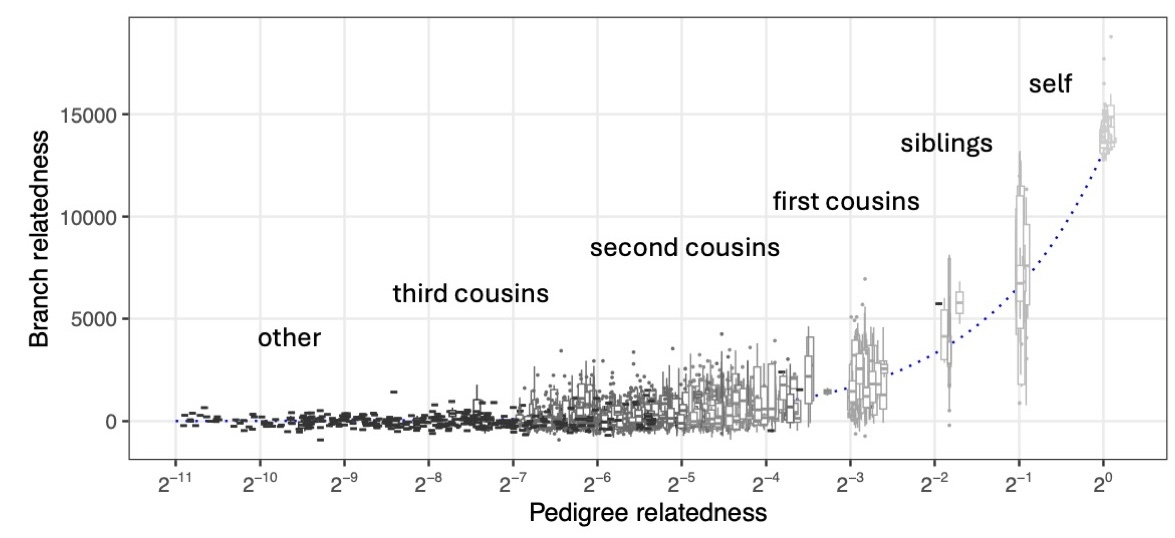
\includegraphics[width=\textwidth]{Figures/Fig5_branch_recap_sim_boxplot_combined_behind2.jpg}
    \caption{Variability in branch relatedness with respect to a fixed pedigree.
    Each box plot corresponds to a pair of individuals with pedigree relatedness
    according to some types of (pedigree) relationships (self, siblings, etc.).
    The box plot for each pair of individuals depicts variation in branch relatedness across 100 ARGs within the fixed pedigree.
    The dotted line indicates the approximate expected branch relatedness,
    which is the pedigree relatedness multiplied by the mean TMRCA among pedigree founders.}
    \label{fig:boxplots}
\end{figure}

% --- EXAMPLE ------------------------------------------------------------

% \subsection{An illustrative example}

% 
\todo[inline]{Update diagram of tree sequence and corresponding notion of relatedness.}
\begin{figure}
    \centering
    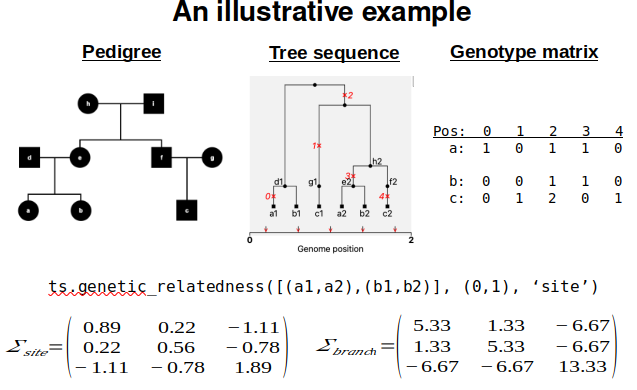
\includegraphics[width=\textwidth]{Figures/ts_gr_example.png}
    \caption{Placeholder for illustrative diagram}
    \label{fig:illustration}
\end{figure}

% \gregor{I think at least one recombination (so we have two local trees) would be nice to have and to connect better to IBD segments.}

% --- GRM computation ----------------------------------------------------

\subsection{Efficient branch GRM-vector products}\label{subsec:matvec}
% JK: I think we can lose this roadmap. Leaving it with 
% you Peter.
We now describe algorithms to compute the branch GRM, showing that it is 
fundamentally a quadratic time operation. Many downstream applications, however,
do not actually require the GRM itself, but instead use the product of the 
GRM times somes vector. We provide a rigorous description of an efficient 
algorithm for this task without forming the branch GRM,
and demonstrate that it has \emph{logarithmic} time complexity.
We then provide an algorithm to compute branch PCA based on this implicit GRM-vector
product used in a randomized SVD method \citep{halko2011findingstructure},
and illustrate its scalability
via simulation-based benchmarks.
The algorithms described are implemented in
the \tskit{} library \citep{ralph2020efficiently, kelleher2024tskit}.

\subsubsection{Computing branch GRM}

As shown in Eq.~\eqref{eqn:divergence_relatedness_branch},
the branch GRM $\mathbf{B}$ is a 
straightforward function of the more fundamental divergence matrix $\mathbf{D}$.
The time complexity of computing the branch GRM is therefore the same as 
the divergence matrix.
The divergence matrix describes
the total branch length separating all $n_S^2$ pairs of samples, such 
that $\mathbf{D}_{i,j} = 2t_u - t_i - t_j$ where $u$ is the MRCA of samples $i$ and $j$.
Because the output is a dense $n_S \times n_S$ matrix 
and at a minimum we must create and fill in the entries of this matrix,
the complexity of this operation is at least $O(n_S^2)$.

So-called ``incremental algorithms'', which use the fact that the 
small changes in tree structure we observe due to recombination events
often correspond to small changes in some accumulated statisic as 
we move along the genome,
have led to very efficient algorithms in several 
contexts~\citep{kelleher2016efficient,ralph2020efficiently,kelleher2020coalescent}. 
The divergence matrix, however, does not easily lend itself to this approach.
Incremental algorithms work well when we only need to consider the effects 
of inserting and removing edges on nodes that are \emph{ancestral to}
a given node. To compute the divergence matrix, however, we need to keep track
of when the MRCAs of each pair of samples change, and this requires 
traversing the subtrees \emph{descending from} nodes affected by 
edges being inserted and removed. Removing (or inserting) an edge changes the MRCA of 
all pairs between the set of samples descending from it 
and those not descending from it. In worst case (removing an edge to the 
root of a balanced binary tree with $n_S$ samples) this involves 
$O(n_S^2)$ work per tree transition, and therefore the complexity of the 
operation is $O(n_T n_S^2)$, where $n_T$ 
is the number of trees along the genome.

The na{\"i}ve approach to this problem 
is to proceed tree-by-tree along the sequence,
iterate over all $\binom{n_S}{2}$ pairs of samples, compute the 
time to their MRCA, and update the corresponding element of $\mathbf{D}$.
MRCAs can be computed efficiently using the Schieber-Vishkin
algorithm \citep{Schieber1988On,knuth2011combinatorial}
which provides the MRCA of two nodes in constant time
after an $O(n_S)$ preprocessing step.
The overall complexity is therefore $O(n_T n_S^2)$,
as we need to perform $O(n_S^2)$ work for all $n_T$ trees.
While this is the same complexity as the incremental approach outlined
above, this ``na{\"i}ve'' approach is in practise much faster, and 
is therefore the implementation used in \tskit{} via the \tsGRM{} method.
\eGRM{} package~\citet{fan2022genealogical} essentially uses the same approach,
although implemented in Python and does not use efficient bulk MRCA queries.
Their approach therefore requires $O(n_T n_S^2 \log^2{n_S})$ time, 
as each MRCA query requires $O$(tree height) time, which is $\log n_S$
if the trees are balanced~\citep{kelleher2016efficient}.
Supplementary Fig~\ref{fig:SI_benchmarking} shows that the \tskit{} implementation 
is faster than the \eGRM{}
implementation~\citep{fan2022genealogical},
% I don't know why this is, but need to acknowledge
although converging for larger sample sizes.

The $O(n_T n_S^2)$ complexity of computing the branch GRM
has significant implications for its utility in large-scale studies:
quadratic algorithms are simply not feasible when we have millions 
of samples.
The approximate mutation-dropping approach of \citet{zhang2023biobank}
is not directly comparable to \citet{fan2022genealogical} and our work.
% JK: trying to distinguish methods here by exact-vs-approximate.
However, their follow-up work with the randomized Haseman-Elston method \citep{zhu2024variance}
indicates that there are scaleable computational approaches that can
work with approximate branch GRMs.
In the next section, we show that it is not necessary
to compute the exact branch GRM explictly in order to \emph{use} it.
For many applications that use the branch GRM we can implicitly compute with it
without materialising the actual matrix.

% and the \ARGneedlelib{} library implements the
% mutation-dropping approach of \citet{zhang2023biobank}.

% % Paragraph on GRM benchmark times
% We found that across a range of settings, our implementation of branch GRM computation,
% \texttt{ts.genetic\_relatedness\_matrix}, outperforms that of the \eGRM{} package
% (Figure~\ref{fig:benchmarking}A,B).
% %
% As expected, the compute time increased with both number of samples and sequence length.
% %
% The relative gap in computation time decreased with the number of sample nodes,
% while remaining stable with the genome sequence length.
% %
% For example, the average time taken to compute the branch GRM
% for $2^9 = 512$ sample nodes was
% 258s for \eGRM{} and 52s for \tsGRM{},
% corresponding to a difference of 3.4 minutes.
% %
% For $2^{12} = 4096$ sample nodes, this difference increased to 11.2 minutes:
% \eGRM{} took on average 86.4 minutes (XYZ seconds) while
% \tsGRM{} took on average 75.2 minutes (XYZ seconds).
% \todo[inline]{Brieuc: This reads very well, but looking at the plot I have to convert all the time, so I suggest adding seconds in brackets.}
% %
% Both implementations reached the memory limit of 4GB
% while computing the GRM for $2^{13}=8192$ sample nodes.

\subsubsection{Computing branch GRM-vector products}
% JK Old version of lead-in. Uncomment to revert

% % Paragraph on matvec for branch GRM via simulating gv
% Many calculations with GRMs involve matrix-vector products
% \citep{colleau2002indirect, colleau2017fast}.

% As a stepping stone towards a scalable branch GRM-vector product algorithm,
% we first present an efficient genetic value simulation algorithm.
% %
% The notation $m \in_{T_k} n$ means that mutation $m$ is on node $n$ at the $k^{\text{th}}$ tree.
% %
% We can write the genetic value of sample $s$ as:
% %
% \begin{align} \label{eqn:genetic_value_trees}
%     Z(s) = \sum_k \sum_{n: s\le_{T_k} n} \sum_{m:m \in_{T_k} n} \beta_m
% \end{align}
% %
% given that $\beta_m$ is the effect size of the derived allele due to $m$.
% %
% Here, we implicitly assume that a child mutation cannot occur at the same site as the parent mutation.

% % Paragraph on pushing mutations down the tree
% Computing $Z(s)$ can be conceptualized as pushing the mutations down the tree.
% %
% We can think of the effect size sums as a weight of a node specific to a local tree,
% motivating the following notation.
% %
% \begin{align}
%     w_k(n) = \sum_{m: m \in_{T_k} n} \beta_m .
% \end{align}
% %
% This term is similar to the weights in \citet{ralph2020efficiently},
% although the resemblance does not play a meaningful role here.
% %
% Unlike the algorithm in \citet{ralph2020efficiently},
% which climbs up the trees from the tips to the root to aggregate the weights of samples,
% computing the value~\eqref{eqn:genetic_value_trees} can be conceptualized as
% pushing the weights from the root down to the samples at the tips.

% % Paragraph on when to push down
% The question for an efficient implementation of this idea
% is when we should push down $w_k(n)$ for each node $n$.
% %
% A brute-force strategy is to do this for every tree.
% %
% However, the sheer number of local trees makes it intractable in large genomes.
% %
% Efficient tree sequence algorithms leverage the shared tree topology
% in adjacent trees to minimize the number of operations.
% %
% In the following Algorithm~\algorithmref{GVSim},
% we only push the weights down when the subtree of the node changes
% as we move from left to right.
% %
% For each node $n$, we have \textit{value} $v(n)$ that collects the genetic effects from above until the subtree changes and
% the \textit{index} $l(n)$ storing the last tree index in which $n$ was updated.

% % The algorithm
% \begin{taocpalg}{GVSim}{Genetic value simulation}
% {
%     Given a sequence of positions that are recombination breakpoints $b_k$ for $1 \le k \le K$ % TODO: we used b for somehing else before
%     along the genome and corresponding sequences of edges to remove ($R_k$) and add ($A_k$) at each position,
%     compute the values
%     \eqref{eqn:genetic_value_trees} for $1 \le s \le n_S$, as long as all samples are leaves in all trees.
%     %
%     Let $T$ be the current tree,
%     initialize $k = 1$, $l(n)=0$, and $v(n) = 0$ for all $n \in \mathbf{V}$.
% }

% \algstep{G1.}{Remove edges}{
%     For each edge $(c, p) \in R_k$,
%     identify the path from $p$ to the root.
%     Move from the root to $p$ along the path.
%     For each $n$ on the path,
%     $v(n) \pluseq \sum_{l=l(n)}^k w_l(n)$ and $l(n)=0$.
%     Then,
%     $v(d) \pluseq v(n)$ for all children $d$ of $n$ and
%     $v(n)=0$.
%     Then,
%     $v(c) \pluseq \sum_{l=l(c)}^k w_l(c)$ and $l(c)=0$.
%     Finally, remove the edge.
% }

% \algstep{G2.}{Add edges}{
%     For each edge $(c, p) \in A_k$,
%     identify the path from $p$ to the root.
%     Move from the root to $p$ along the path.
%     For each $n$ on the path,
%     $v(n) \pluseq \sum_{l=l(n)}^k w_l(n)$ and $l(n)=0$.
%     Then,
%     $v(d) \pluseq v(n)$ for all children $d$ of $n$ and
%     $v(n)=0$.
%     Then, $l(c)=0$.
%     Finally, add the edge.
% }

% \algstep{G3.}{Iteration}{
%     If $k < N$,
%     set $k = k + 1$ and return to \algorithmref{\textbf{V1}}.
%     Otherwise, set $z_s = v(s)$ for $1 \le s \le n_S$ and finish.
% }

% \end{taocpalg}

% % Paragraph on describing the algorithm
% The algorithm only adds the genetic values from above to its child when the subtree changes.
% %
% This saves the number of operations compared to pushing things down for every tree
% because most edges remain the same between close trees.
% %
% Next, it ensures that a mutation's effect is passed down to the correct samples
% because the genetic effects that nodes have accumulated
% are passed down just before the samples beneath them change due to an edge insertion or deletion.
% %
% After passing the previously accumulated genetic effects,
% $v(n)$ is set to zero and starts collecting genetic values for the new set of samples.
% %
% This is why we have to track $l(\cdot)$ to remember the last time the node was updated,
% as we should only send genetic values that has not yet been passed to the child.
% %
% Hence, we can say that the algorithm \textit{lazily} passes
% the genetic values from the root to the tips only when it is necessary;
% when the samples below a node changes.
% %
% In other words, sending genetic values from above to below before the subtree change is redundant,
% and not doing so when the subtree changes will pass the values to the wrong samples.

Many calculations with GRMs involve matrix-vector products
\citep{colleau2002indirect, colleau2017fast}. The straightforward way is
to first compute the GRM, and to then compute its product with 
the vector in question. This places strong limits on the size of the 
datasets that we can work with, due to quadratic space and time complexity
in the number of samples, $n_S$. In certain situations, however, 
given that the output of an $(n\times n)$-matrix times an $n$-vector is,
itself an $n$-vector, we can perform this calculation without explicitly
materialising the matrix, thus avoiding the quadratic space complexity.
In rarer situations, we can even exploit the structure of the matrix to 
also avoid the quadratic \emph{time} complexity. Not only do we not fully
materialise the matrix in memory, we never actually compute all $n_S^2$
elements of the matrix. Here, we develop an algorithm of the 
latter form, which allows us to exactly compute the product of the 
branch GRM with an arbitrary vector in substantially less time than
it would take to compute the matrix itself.

To do this we require some notation.
Suppose that $\mathbf{C}_{s,t}$ is an uncentered branch relatedness between
sampled genomes $s$ and $t$ as computed from the trees, that is,
the sum of the areas of all branches in all trees that are ancestral to both $s$ and $t$.
% TODO: we used b for somehing else before
\begin{align} \label{defn:pairwise_relatedness}
    \mathbf{C}_{s,t} = \sum_k (b_k - b_{k-1}) \sum_{n: s,t \le_{T_k} n} \ell_{T_k}(n) % TODO: what is \ell_{T_k} here?
\end{align}
For a given vector $\mathbf{w}$, we'd like to compute the matrix-vector product $\mathbf{C}\mathbf{w}$.
Suppose that $b_k$ ($k=0,\ldots,K$) are the recombination breakpoints on the genome
including the start and end of the genome (the genome is a closed interval $[b_0, b_K]$).
Suppose that the $k^{\text{th}}$ tree $T_k$ extends over a span $b_k - b_{k-1}$ along the genome,
that the length of the edge (in units of time) above node $n$ in $T_k$ is $\ell_{T_k}(n) = t_{p(n)}-t_n$,
where $p(n)$ is the parent node of $n$.
The partial ordering $\le_T$ of nodes are induced by the tree that older nodes are larger than the younger nodes.

% Paragraph on computing the matrix-vector product
The $s^{\text{th}}$ element of the matrix-vector product $\mathbf{C}\mathbf{w}$ is:
\begin{align} \label{eq:similar_ralph2020}
    \begin{aligned}
        (\mathbf{C}\mathbf{w})_s &=
        \sum_t \mathbf{C}_{s,t} w_t \\
        &=
        \sum_t
        \left(
            \sum_k (b_k - b_{k-1}) \sum_{n: s,t \le_{T_k} n} \ell_k(n)
        \right) {w}_t \\
        &=
        \sum_k (b_k - b_{k-1})
        \sum_t
        \sum_{n: s,t \le_{T_k} n} \ell_{T_k}(n) {w}_t \\
        &=
        \sum_k (b_k - b_{k-1})
        \sum_{n: s\le_{T_k} n} \ell_{T_k}(n)
        \sum_{t:t \le_{T_k} n} {w}_t \\
        &=
        \sum_k (b_k - b_{k-1})
        \sum_{n: s\le_{T_k} n} \ell_{T_k}(n) w_k(n)
    \end{aligned}
\end{align}
The new variable $w_k(n)$ is the sum of sample weights below $n$ in tree $T_k$:
\begin{align}
    w_k(n) = \sum_{t:t \le_{T_k} n} {w}_t ,
\end{align}
which is a familiar term from \citet{ralph2020efficiently}.
Although a single entry of $\mathbf{C}\mathbf{w}$ could be computed efficiently
from the algorithm in \citet{ralph2020efficiently},
it doesn't scale well because it requires a separate set of weights for 
each entry of the vector.

% We can see from equation~\eqref{eq:similar_ralph2020} that $\mathbf{C}\mathbf{w}$ is
% a sum of the contributions $\ell_{T_k}(n)w_k(n)$ of nodes specific to local trees.
% Adding these contributions directly to the entries of $\mathbf{C}\mathbf{w}$ is
% inefficient due to the sheer number of node and sample pairs.
% We can mitigate this by pushing down the contribution of the nodes only to their adjacent child nodes at a time,
% in the hope that the contributions will be passed to the correct samples corresponding to the entries of $\mathbf{C}\mathbf{w}$.
% This is because the local connection between the nodes is extremely sparse in the tree sequence.
% The role of value $v(\cdot)$ is precisely to deliver the contributions correctly downwards the trees.
% For each tree $T_k$, we want to ensure that $n$'s contribution is passed down only to
% the samples $s$ such that $s \le_{T_k} n$.
% A straightforward way is to pass down the contributions at every position $k$.

% Paragraph on efficient way of computing the matrix-vector product
We present an efficient algorithm for computing the entire matrix-vector product.
The general idea is simple: as we move left-to-right along the tree sequence,
we keep track of two things for each node $n$:
the \textit{weight} $w(n)$ of the node in the current tree ($w_k(n)$ above) and
the \textit{value} $v(n)$ of the haplotype carried by $n$,
which will contribute to all descendants of $n$.
 % (we will explain the role of $v(\cdot)$ in detail shortly).
Additionally, we keep track of the last \textit{position} $x(n)$ in which the node was updated.
As we move along the genome, we update any nodes ancestral to any changes in the tree:
all other nodes are the roots of unchanged subtrees and hence remains unchanged.
As seen above, each branch contributes to potentially many entries in the output vector,
so by accumulating values of haplotypes, we reduce the amount of necessary work.

% The algorithm that is used in practice is a modification of the one that we presented in the main paragraphs.
% $v(n)$ does not retain its previous interpretation of values that $n$ has inherited from its ancestors
% but has not yet passed down to its descendants.
% The algorithm looks simpler at a glance but requires a more careful read to understand.

\begin{taocpalg}{V}{Branch GRM-vector product}
{
    Given a sequence of positions that are recombination breakpoints $b_k$ for $1 \le k \le K$ 
    along the genome and corresponding sequences of edges to 
    remove ($R_k$) and add ($A_k$) at each position, 
    compute the values 
    $y_s=\sum_t\mathbf{C}_{st} w_t$ for $1 \le s \le n_S$, assuming all samples are leaves in all trees.
    Let $T$ be the current tree,
    $\ell_T(n) = t_{p(n)} - t_n$ be the length of the branch above $n$ in $T$ (or zero, if $n$ has no parent),
    initialize $k = 1$, $x(n) = 0$, and $v(n) = 0$ for all $n \in \mathbf{V}$.
    Set $w(s) = w_s$ for each sample $s$, and $w(n)=0$ for all other nodes.
    % Is this correct Peter? This really confused me for a while, using the 
    % same notation for arrays we're storing and functions.
    Let $z(n) = \ell_{T_k}(n) (b_k - x(n))$ be a function 
    computed from the current values of $k$ and $x$ at all times.
}

\algstep{V1.}{Remove edges}{
    For each edge $(c, p) \in R_k$,
    and for each node $n \ge_T p$,
    set $v(n) \pluseq z(n)w(n)$,
    then
    $w(n) \minuseq w(c)$, 
    $v(c) \pluseq v(n)$,
    and $x(n) = b_k$.
    Then, set $x(c) = b_k$
    and remove the edge.
}

\algstep{V2.}{Add edges}{
    For each edge $(c, p) \in A_k$,
    and for each node $n \ge_T p$,
    set $v(n) \pluseq z(n)w(n)$,
    then
    $w(n) \pluseq w(c)$,
    $v(c) \minuseq v(n)$,
    and $x(n) = b_k$.
    Then, set $x(c) = b_k$
    and add the edge.
}

\algstep{V3.}{Iteration}{
    If $k < N$,
    set $k \pluseq 1$ and return to \algorithmref{\textbf{V1}}.
    Otherwise, set $y_s = v(s)$ for $1 \le s \le n_S$ and finish.
}

\end{taocpalg}

% The simplified algorithm; this was moved in here to give us less to explain
% and fewer opportunities to confuse readers as to what we're doing.
% The vast majority of readers aren't going to understand the simpler algorithm 
% anyway, so no point in confusing them more.
% % The algorithm
% \begin{taocpalg}{bGRM-vec}{Branch GRM-vector}
% {
%     Given a sequence of positions that are recombination breakpoints $b_k$ for $1 \le k \le K$
%     along the genome and corresponding sequences of edges to remove ($R_k$) and add ($A_k$) at each position,
%     compute the values
%     $y_s=\sum_t\mathbf{C}_{st} w_t$ for $1 \le s \le n_S$, as long as all samples are leaves in all trees.
%     %
%     Let $T$ be the current tree,
%     $\ell_T(n) = t_{p(n)} - t_n$ be the length of the branch above $n$ in $T$ (or zero, if $n$ has no parent),
%     initialize $k = 1$, $x(n) = 0$, and $v(n) = 0$ for all $n \in \mathbf{V}$.
%     Set $w(s) = w_s$ for each sample $s$, and $w(n)=0$ for all other nodes.
%     At all times, define
%     $z(n) = \ell_{T_k}(n) (b_k - x(n)) $ where $T_k$ is the current tree.
% }

% \algstep{V1.}{Remove edges}{
%     For each edge $(c, p) \in R_k$,
%     identify the path from $p$ to the root.
%     Move from the root to $p$ along the path.
%     For each $n$ on the path,
%     $v(n) \pluseq z(n)w(n)$ and
%     $x(n)=b_k$.
%     Then,
%     $v(d) \pluseq v(n)$ for all children $d$ of $n$ and
%     $v(n)=0$.
%     Then,
%     $v(c) \pluseq z(c)w(c)$ and set $x(c)=b_k$.
%     Move from $p$ to the root along the path.
%     For each $n$ on the path,
%     $w(n) \minuseq w(c)$.
%     Finally, remove the edge.
% }

% \algstep{V2.}{Add edges}{
%     For each edge $(c, p) \in A_k$,
%     identify the path from $p$ to the root.
%     Move from the root to $p$ along the path.
%     For each $n$ on the path,
%     $v(n) \pluseq z(n)w(n)$ and
%     $x(n)=b_k$.
%     Then,
%     $v(d) \pluseq v(n)$ for all children $d$ of $n$ and
%     $v(n)=0$.
%     Then,
%     $x(c)=b_k$.
%     Move from $p$ to the root along the path.
%     For each $n$ on the path,
%     $w(n) \pluseq w(c)$.
%     Finally, add the edge.
% }

% \algstep{V3.}{Iteration}{
%     If $k < N$,
%     set $k = k + 1$ and return to \algorithmref{\textbf{V1}}.
%     Otherwise, set $y_s = v(s)$ for $1 \le s \le n_S$ and finish.
% }

% \end{taocpalg}

Algorithm~\algorithmref{V} follows a similar structure to previous incremental 
algorithms~\citep{kelleher2016efficient,ralph2020efficiently}:
at each tree transition we update some global state to account for the 
insertion and removal of the edges affected. Here, the overall 
goal is different: rather than keeping track of some cumulative value
among the nodes in a given subtree (say, total branch length) we are instead
keeping track of the total contribution to each node from nodes
\emph{ancestral to it}.
By some subtle bookkeeping, we can keep track of the cumulative 
contribution to each node, in only updating each node when 
it is affected by an edge insertion or removal.
% Notice that the samples below a node do not change until the subtree beneath it changes.
% This change is triggered by edge insertions and deletions happening below the edge,
% so we wait until the change happens.
Each node accumulates the contributions that are passed down from above
until an edge below it is added or removed.
At each edge insertion or removal $v(n)$ is updated by traversing up
to the root of the current subtree (also keeping the weights $w(n)$
up to date), and the accumulated 
contribution passed down to the child node of the edge $c$.
Finally, we set $x(c)$ is set to $b_k$ (the current position) to mark
the last position this node was updated.

The above explanation is a rough sketch of the algorithm.
A full proof of correctness is provided in Appendix~\ref{sec:proof-algv-correct}.
The algorithm has been implemented in the \tsGRMv{} % \texttt{ts.genetic\_relatedness\_vector}
in \tskit{}, and is extensively tested.

% After passing down $v(n)$, it is set to $0$ and $x(n)$ is set to $b_k$ (the current position).
% Then, $v(n)$ repeats to accumulate the contributions from above, including itself,
% for the newly updated set of samples.
% Lastly, we add or subtract the weights of $c$ from the nodes above similarly to
% the algorithm in \citet{ralph2020efficiently} to keep the weights up-to-date.

% JK: These notes belong in the explanation bit, maybe?
% % Paragraph on the efficiency of the algorithm
% The algorithm is efficient because the operations occur locally between adjacent nodes in the tree sequence.
% %
% We can also see that the nodes in the path from the inserted/deleted edge to the root are
% modified to keep the computation minimal.
% %
% It passes the contributions $\ell_{T_k}(n)w_k(n)$ correctly because
% $v(\cdot)$ is passed down whenever the subtree changes.
% %
% From this point of view, we can interpret $v(\cdot)$ as the sum of contributions that $n$ inherited from above,
% but had not yet has been sent to the nodes and samples below in the previous trees.

\begin{figure}
    \centering
    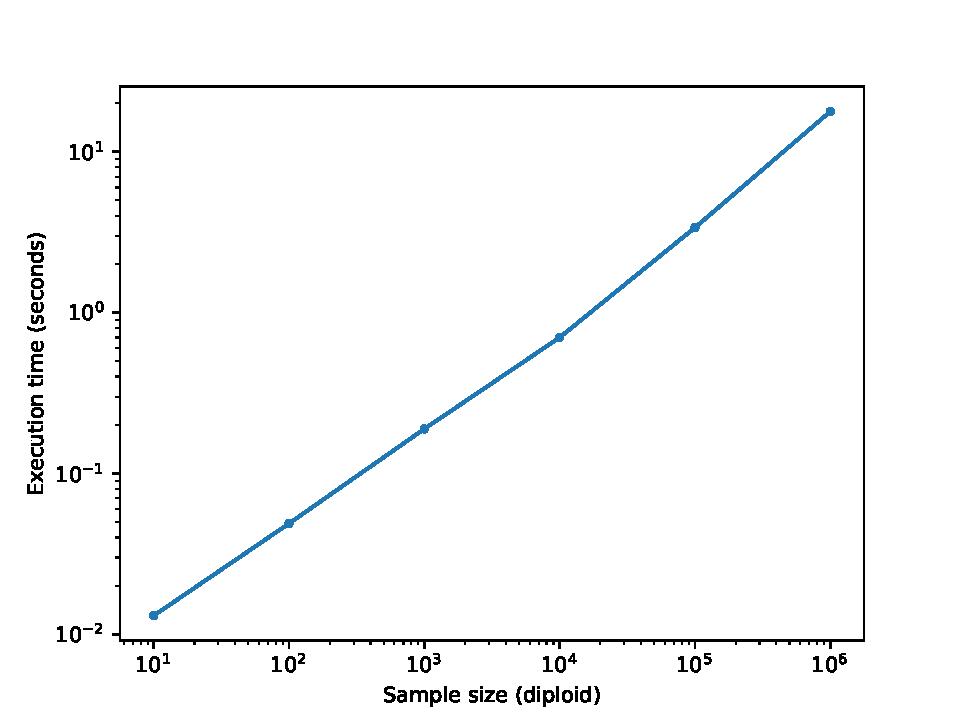
\includegraphics[width=5cm]{Figures/matvec-benchmark}
    \caption{Computational scaling of the branch GRM-vector product algorithm
    implemented in \tskit{} for subsets of a large simulation 
    of French-Canadians.
    \label{fig:matvec-benchmark}}
\end{figure}

The analysis of this algorithm is straightforward and follows a standard 
pattern~\citep{kelleher2016efficient,ralph2020efficiently}. Because
recombination results in a small modification of the current tree,
each tree transition
incurs $O(1)$ edge removals and insertions. Each edge removal in step \textbf{V1}
involves examining only nodes ancestral to the edge, and therefore incurs
a cost of $O(\log{n_S})$, assuming trees are balanced. Edge insertions
in \textbf{V2} have the same cost. Thus, 
as the first tree requires inserting $O(n_S)$ edges requiring $O(1)$
work, the overall complexity is $O(n_S + n_T \log{n_S})$.
This logarithmic time complexity is borne out in
Figure~\ref{fig:matvec-benchmark} where we plot the time taken to compute the 
branch GRM-vector product against subsets of a large simulated
ARG~\citep{andersontrocme2023genes}. Here, it takes only
17.8 seconds to run the \tsGRMv{} method 
on the ARG with 1 million diploid samples
(6,694,080 nodes; 31,840,754 edges; 4,013,273 trees).
In contrast, computing the full branch
GRM using the \tsGRM{} method 
for the ARG with ten diploid samples
% This is too slow - I think the implementation could be improved quite a lot
% by minimising the oriented forest we pass to the SV algorithm. We're currently
% passing the full 61K nodes in, resulting in a lot of memory getting shuttled
% around.
(61,412 nodes;  297,171 edges; 93,543 trees) required 28 seconds.

% --- PCA ----------------------------------------------------------------

\subsubsection{Branch PCA}

We found the principal components (PCs) of the branch GRM
using a randomized SVD \citep{halko2011findingstructure},
a method that can find the
eigenvectors of a matrix that is only implicitly defined through a matrix-vector multiplication.
Algorithm~\algorithmref{rPCA} explains this process.

\begin{taocpalg}{rPCA}{Randomized PCA of branch GRM}
{
    Let $\mathbf{C}$ be the branch GRM for $n_I$ individuals,
    let $k$ be the desired number of PCs, and $q$ the number of iterations.
    Multiplying $\mathbf{C}$ with a vector is done by Algorithm~\algorithmref{\textbf{V}}.
}
    
\algstep{P1.}{Range estimation}{
    Sample a random matrix $\boldsymbol{\Omega} \in \mathbb{R}^{n_I \times k}$ in which the entries are independent standard normal variables.
    Obtain a basis matrix $\mathbf{Q} \in \mathbb{R}^{n_I \times k}$ by applying QR decomposition to $\mathbf{C}\boldsymbol{\Omega}$.
    Repeat $q$ times, updating the basis matrix $\mathbf{Q}$
    by applying QR decomposition to $\mathbf{C}\mathbf{Q}$,
    where $\mathbf{Q}$ is from the previous iteration.
}

\algstep{P2.}{Small singular value decomposition}{
    Compute $\mathbf{W} = \mathbf{Q}^\intercal \mathbf{C}$ and obtain
    the singular vector $\mathbf{U} \in \mathbb{R}^{k \times k}$
    by exact singular value decomposition of $\mathbf{W}$.
    Then the columns of $\mathbf{Q}\mathbf{U} \in \mathbb{R}^{n \times k}$
    contain the desired PCs of the branch GRM $\mathbf{C}$.
}

\end{taocpalg}

The algorithm has two advantages over directly applying the exact SVD to the branch GRM.
%
It needs less time and memory because the $n_I \times n_I$ branch GRM is never computed nor stored.
%
The algorithm extracts the relevant information through
the efficient matrix-vector product Algorithm~\algorithmref{V}.
%
Secondly, the exact SVD is applied to an $n_I \times k$ matrix,
where $k$ is much smaller than $n_I$.
%
This reduces the amount of computation considerably.

\begin{figure}
    \centering
    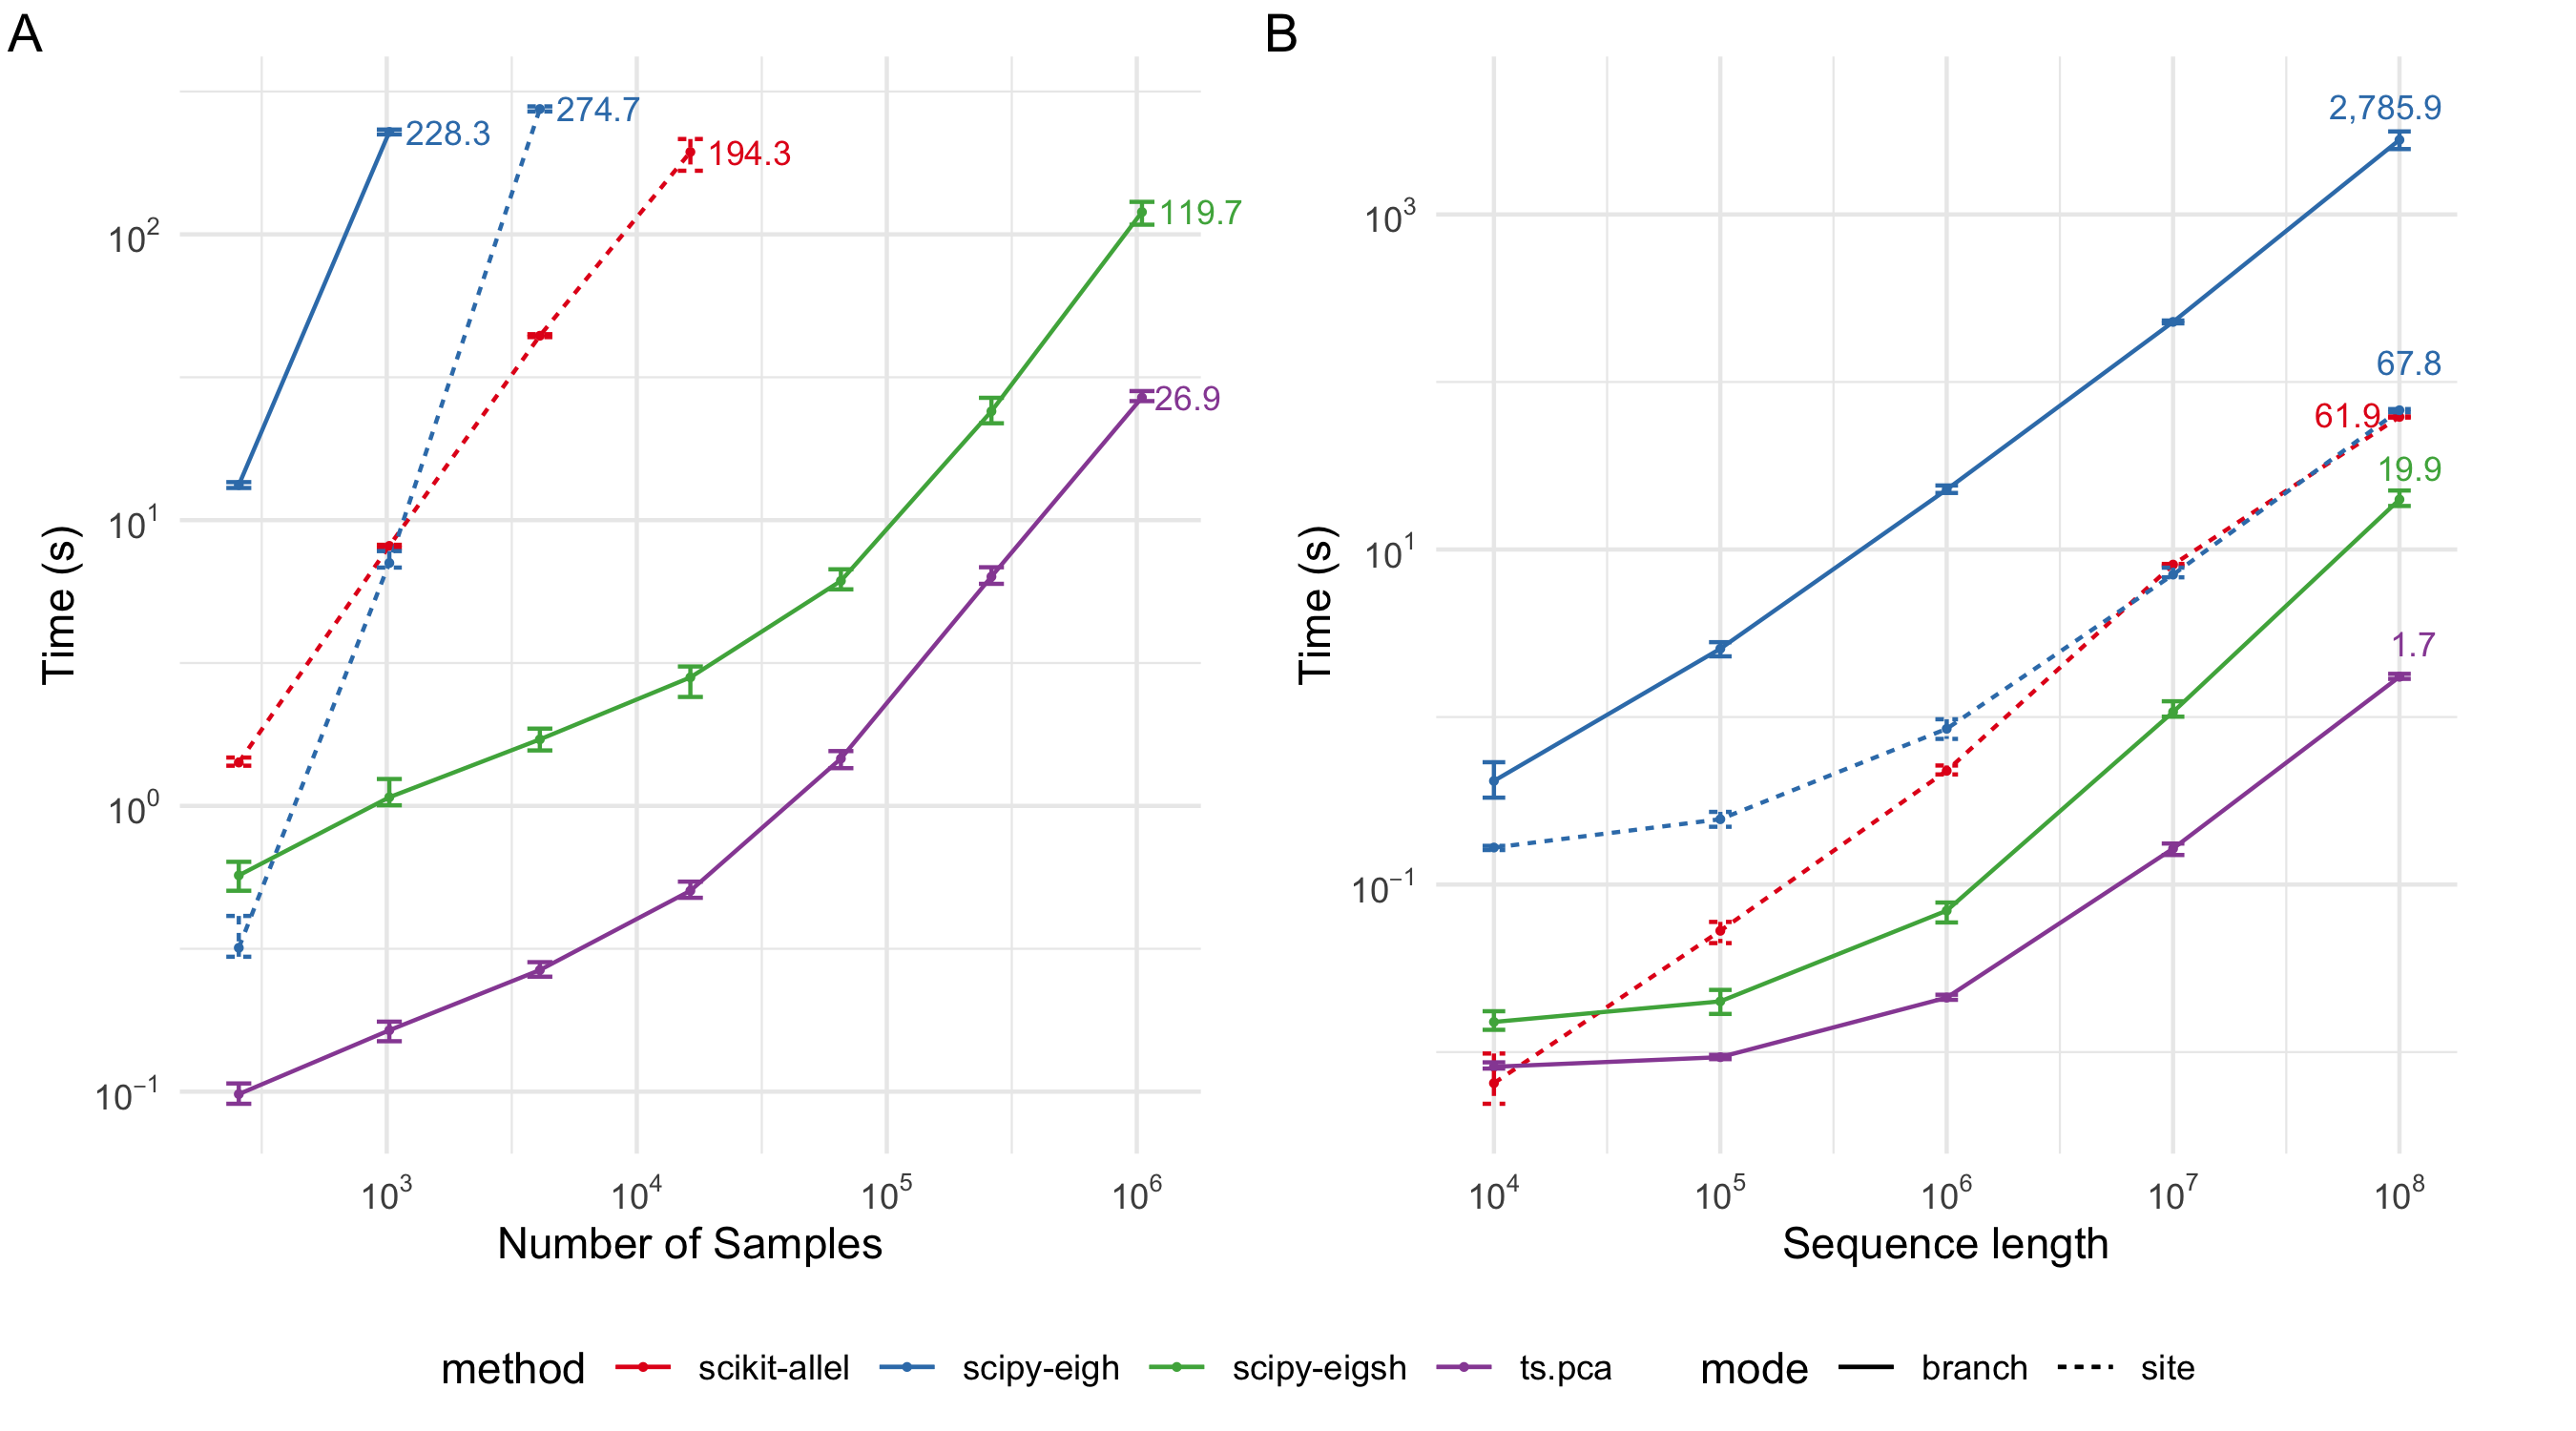
\includegraphics[width=\textwidth]{Figures/Fig2_benchmarking_plot.png}
    \caption{Time efficiency of different implementations of PCA computations.
    Each dot corresponds to the average time taken across ten simulations with different random seeds.
    Error bars represent the range in time taken across the ten simulations.
    (A) PCA with genome sequence length fixed at $10^{7}$ and varying the number of samples.
    (B) PCA with number of sample nodes fixed at $2^{10}$ and varying genome sequence length.
    Branch mode refers to branch PCA and site mode refers to genotype PCA.
    \label{fig:benchmarking}}
\end{figure}

The efficiency of the branch PCA algorithm
and the underlying branch GRM-vector product algorithm is illustrated in
Figure~\ref{fig:benchmarking}. 
See Methods for details of the benchmarking methodology.
% Paragraph on PCA benchmark times
For PCA, we observed significant benefits from using implementations that avoided the storage of the GRM or genotype matrix in memory,
particularly for larger numbers of samples (Figure~\ref{fig:benchmarking}).
%
Notably, \tsGRM{} failed due to memory limits
when computing the branch GRM for $2^{12} = 4096$ sample nodes and
when computing the genotype (site) GRM for $2^{14} = 16384$ sample nodes.
%
Implementation of randomized PCA on genotype matrix in \scikitallel{}
failed due to memory limits for $2^{16} = 65536$ sample nodes.
%
Notwithstanding, the implementations that relied solely on
the implicit matrix-vector product using \tskit{} were substantially more efficient.
%
Specifically, both \tsPCA{} and \eigsh{} from \scipy{} using \tsGRMv{} % not \tsGRMw{}!?
as a linear operator were able to scale to $2^{20} = 1,048,576$ samples.
%
The native implementation of \tsPCA{} consistently outperformed \eigsh{},
with the relative difference decreasing slightly with the number of samples, and increasing with sequence length.
%
Moreover, the difference in absolute compute time increased with both sample size and sequence length.
%
For example, \tsPCA{} took on average
0.27s for $2^{12} = 4,096$ samples and
26.9s for $2^{20} = 1,048,576$ samples,
while \eigsh{} took
  1.7s for $2^{12} = 4,096$ samples and
119.7s for $2^{20} = 1,048,576$ samples.
%
This difference primarily reflects the differences in the underlying algorithms used for PCA:
\tsPCA{} uses a randomized SVD while
\eigsh{} uses the implicitly restarted Lanczos method \citep{lehoucq1998arpack}.